\item \subquestionpoints{5}
Investigate why the training procedure behaves unexpectedly on dataset $B$, but
not on $A$. Provide hard evidence (in the form of math, code, plots, etc.) to
corroborate your hypothesis for the misbehavior. Remember, you should address
why your explanation does \emph{not} apply to $A$.

\textbf{Hint}: The issue is not a numerical rounding or over/underflow error.

\ifnum\solutions=1 {
  \begin{answer}

    For $y\in\{1, -1\}$, 
    $$
    \begin{aligned}
        p(y = 1\mid x;\theta) &= h_\theta(x) = \frac{1}{1 + e^{-\theta^T x^{(i)}}}   \\
        p(y = -1\mid x;\theta) &= 1 - h_\theta(x) = 1 - \frac{1}{1 + e^{-\theta^T x^{(i)}}} = \frac{1}{1 + e^{\theta^T x^{(i)}}}\\
        \therefore p(y\mid x;\theta) &= \frac{1}{1 + e^{-y^{(i)} \theta^T x^{(i)}}}\\
    \end{aligned}
    $$
    So the log likelihood of $\theta$ is
    $$
    \begin{aligned}
        \ell(\theta) &= \log{L(\theta)}\\
        &= \log\left(\prod_{i=1}^n p(y\mid x;\theta)\right)\\
        &= -\sum_{i=1}^n\log\left(1 + e^{-y^{(i)}\theta^T x^{(i)}}\right) \\
    \end{aligned}
    $$
    Instead of maximazing $\ell(\theta)$, we minimize the lose function
    $$
    J(\theta) = \sum_{i=1}^n\log\left(1 + e^{-y^{(i)}\theta^T x^{(i)}}\right) \\
    $$
    note that $y^{(i)}\theta^T x^{(i)}$ is the functional margin(we add a 1 in each $x^{(i)}$, 
    so it's equivalent to $y^{(i)}(w^Tx^{(i)}+b)$),when the dataset is linearly separable, 
    then $\exists\ \theta,\forall\ x^{(i)}, y^{(i)}\theta^T x^{(i)} > 0$. Therefore if you mutiply 
    $\theta$ by some large scalar, the separating hyperplane remains the same, but $J(\theta)$ is 
    smaller($\theta$ is bigger, $y^{(i)}\theta^T x^{(i)}$ is bigger, $e^{-y^{(i)}\theta^T x^{(i)}}$ 
    is smaller, $\log(1 + e^{-y^{(i)}\theta^T x^{(i)}})$ is smaller). In this case, in order to 
    minimize the lose function, $\theta$ will be bigger and bigger and the algrithm cannot converge.

    However, when the dataset isn't linearly separable, then $\exists x^{(i)},y^{(i)}\theta^T x^{(i)} < 0$.
    If you continue to increase $\theta$, then $e^{-y^{(i)}\theta^T x^{(i)}}$ will be bigger and bigger, 
    so is $J(\theta)$. Therefore, in this case, there must be some optimal $\theta$ to make the algorithm converge.
    \begin{figure}[htbp]
        \centering
        \begin{minipage}[t]{0.48\textwidth}
            \centering
            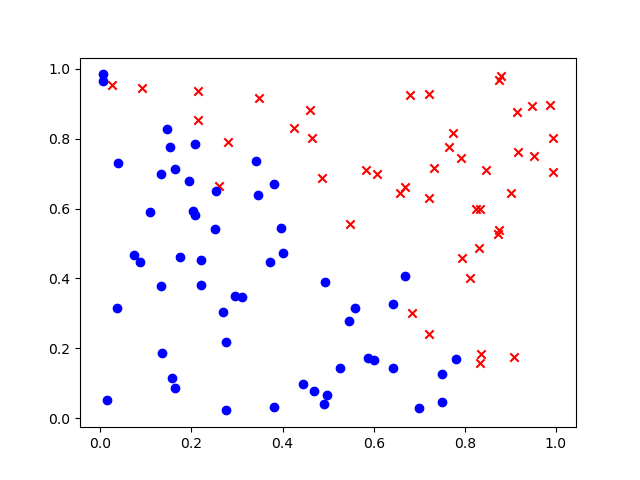
\includegraphics[width=6cm]{../src/output/dataset1_a.png}
            \caption{dataset A isn't linearly separable}
        \end{minipage}
        \centering
        \begin{minipage}[t]{0.48\textwidth}
            \centering
            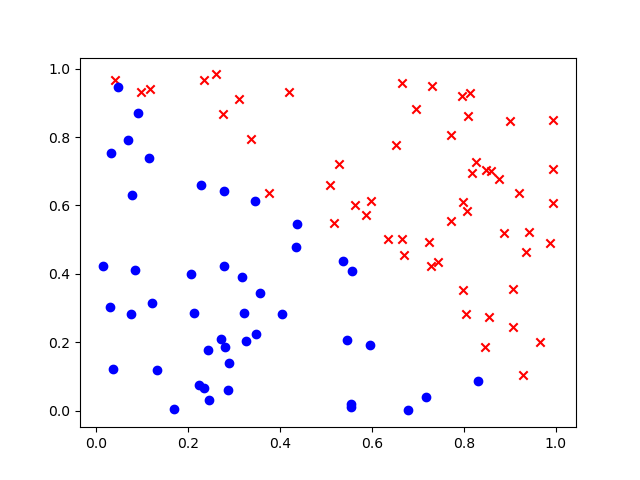
\includegraphics[width=6cm]{../src/output/dataset1_b.png}
            \caption{dataset B is linearly separable}
        \end{minipage}
    \end{figure}
\end{answer}

} \fi
